%===============================================================================
% LaTeX sjabloon voor de bachelorproef toegepaste informatica aan HOGENT
% Meer info op https://github.com/HoGentTIN/latex-hogent-report
%===============================================================================

\documentclass[dutch,dit,thesis]{hogentreport}

% TODO:
% - If necessary, replace the option `dit`' with your own department!
%   Valid entries are dbo, dbt, dgz, dit, dlo, dog, dsa, soa
% - If you write your thesis in English (remark: only possible after getting
%   explicit approval!), remove the option "dutch," or replace with "english".

\usepackage{lipsum} % For blind text, can be removed after adding actual content

%% Pictures to include in the text can be put in the graphics/ folder
\graphicspath{{../graphics/}}

%% For source code highlighting, requires pygments to be installed
%% Compile with the -shell-escape flag!
%% \usepackage[chapter]{minted}
%% If you compile with the make_thesis.{bat,sh} script, use the following
%% import instead:
\usepackage[chapter,outputdir=../output]{minted}
\usemintedstyle{solarized-light}

%% Formatting for minted environments.
\setminted{%
    autogobble,
    frame=lines,
    breaklines,
    linenos,
    tabsize=4
}

%% Ensure the list of listings is in the table of contents
\renewcommand\listoflistingscaption{%
    \IfLanguageName{dutch}{Lijst van codefragmenten}{List of listings}
}
\renewcommand\listingscaption{%
    \IfLanguageName{dutch}{Codefragment}{Listing}
}
\renewcommand*\listoflistings{%
    \cleardoublepage\phantomsection\addcontentsline{toc}{chapter}{\listoflistingscaption}%
    \listof{listing}{\listoflistingscaption}%
}

% Other packages not already included can be imported here

%%---------- Document metadata -------------------------------------------------
% TODO: Replace this with your own information
\author{Ernst Aarden}
\supervisor{Dhr. F. Van Houte}
\cosupervisor{Mevr. S. Beeckman}
\title[Optionele ondertitel]%
    {Titel van de bachelorproef}
\academicyear{\advance\year by -1 \the\year--\advance\year by 1 \the\year}
\examperiod{1}
\degreesought{\IfLanguageName{dutch}{Professionele bachelor in de toegepaste informatica}{Bachelor of applied computer science}}
\partialthesis{false} %% To display 'in partial fulfilment'
%\institution{Internshipcompany BVBA.}

%% Add global exceptions to the hyphenation here
\hyphenation{back-slash}

%% The bibliography (style and settings are  found in hogentthesis.cls)
\addbibresource{bachproef.bib}            %% Bibliography file
\addbibresource{../voorstel/voorstel.bib} %% Bibliography research proposal
\defbibheading{bibempty}{}

%% Prevent empty pages for right-handed chapter starts in twoside mode
\renewcommand{\cleardoublepage}{\clearpage}

\renewcommand{\arraystretch}{1.2}

%% Content starts here.
\begin{document}

%---------- Front matter -------------------------------------------------------

\frontmatter

\hypersetup{pageanchor=false} %% Disable page numbering references
%% Render a Dutch outer title page if the main language is English
\IfLanguageName{english}{%
    %% If necessary, information can be changed here
    \degreesought{Professionele Bachelor toegepaste informatica}%
    \begin{otherlanguage}{dutch}%
       \maketitle%
    \end{otherlanguage}%
}{}

%% Generates title page content
\maketitle
\hypersetup{pageanchor=true}

%%=============================================================================
%% Voorwoord
%%=============================================================================

\chapter*{\IfLanguageName{dutch}{Woord vooraf}{Preface}}%
\label{ch:voorwoord}

%% TODO:
%% Het voorwoord is het enige deel van de bachelorproef waar je vanuit je
%% eigen standpunt (``ik-vorm'') mag schrijven. Je kan hier bv. motiveren
%% waarom jij het onderwerp wil bespreken.
%% Vergeet ook niet te bedanken wie je geholpen/gesteund/... heeft

\lipsum[1-2]
%%=============================================================================
%% Samenvatting
%%=============================================================================

% TODO: De "abstract" of samenvatting is een kernachtige (~ 1 blz. voor een
% thesis) synthese van het document.
%
% Een goede abstract biedt een kernachtig antwoord op volgende vragen:
%
% 1. Waarover gaat de bachelorproef?
% 2. Waarom heb je er over geschreven?
% 3. Hoe heb je het onderzoek uitgevoerd?
% 4. Wat waren de resultaten? Wat blijkt uit je onderzoek?
% 5. Wat betekenen je resultaten? Wat is de relevantie voor het werkveld?
%
% Daarom bestaat een abstract uit volgende componenten:
%
% - inleiding + kaderen thema
% - probleemstelling
% - (centrale) onderzoeksvraag
% - onderzoeksdoelstelling
% - methodologie
% - resultaten (beperk tot de belangrijkste, relevant voor de onderzoeksvraag)
% - conclusies, aanbevelingen, beperkingen
%
% LET OP! Een samenvatting is GEEN voorwoord!

%%---------- Nederlandse samenvatting -----------------------------------------
%
% TODO: Als je je bachelorproef in het Engels schrijft, moet je eerst een
% Nederlandse samenvatting invoegen. Haal daarvoor onderstaande code uit
% commentaar.
% Wie zijn bachelorproef in het Nederlands schrijft, kan dit negeren, de inhoud
% wordt niet in het document ingevoegd.

\IfLanguageName{english}{%
\selectlanguage{dutch}
\chapter*{Samenvatting}
\lipsum[1-4]
\selectlanguage{english}
}{}

%%---------- Samenvatting -----------------------------------------------------
% De samenvatting in de hoofdtaal van het document

\chapter*{\IfLanguageName{dutch}{Samenvatting}{Abstract}}

\lipsum[1-4]


%---------- Inhoud, lijst figuren, ... -----------------------------------------

\tableofcontents

% In a list of figures, the complete caption will be included. To prevent this,
% ALWAYS add a short description in the caption!
%
%  \caption[short description]{elaborate description}
%
% If you do, only the short description will be used in the list of figures

\listoffigures

% If you included tables and/or source code listings, uncomment the appropriate
% lines.
\listoftables

\listoflistings

% Als je een lijst van afkortingen of termen wil toevoegen, dan hoort die
% hier thuis. Gebruik bijvoorbeeld de ``glossaries'' package.
% https://www.overleaf.com/learn/latex/Glossaries

%---------- Kern ---------------------------------------------------------------

\mainmatter{}

% De eerste hoofdstukken van een bachelorproef zijn meestal een inleiding op
% het onderwerp, literatuurstudie en verantwoording methodologie.
% Aarzel niet om een meer beschrijvende titel aan deze hoofdstukken te geven of
% om bijvoorbeeld de inleiding en/of stand van zaken over meerdere hoofdstukken
% te verspreiden!

%%=============================================================================
%% Inleiding
%%=============================================================================

\chapter{\IfLanguageName{dutch}{Inleiding}{Introduction}}%
\label{ch:inleiding}

% Waar gaat het onderzoek over?
Softwareframeworks zoals Angular vereenvoudigen het maken van dynamische webapplicaties.
Zoals vele software krijgt Angular geregeld updates.
Deze updates komen met verschillende voordelen, zoals: nieuwe functionaliteiten, betere performantie, bugfixes, \dots.
Het toepassen van deze updates is niet altijd even vanzelfsprekend.
Soms dienen nieuwe functionaliteiten als vervanging voor oudere functionaliteiten.
Dit zorgt ervoor dat de code die Angular aanspreekt ook moet veranderen.

% Wat is de context?
Het bedrijf Stater is een end-to-end dienstverlener voor zowel hypothecaire als consumentenkredieten.
Ze ondersteunen de kredietverstrekker voor de dienstverlening aan consumenten.
Stater heeft intern meerdere applicaties die gebruikmaken van het Angular-framework.
Specifiek gebruiken deze applicaties Angular versie 16 (v16).
Stater zou graag al deze applicaties updaten naar de meest recente versie, Angular versie 20 (v20).

\section{\IfLanguageName{dutch}{Probleemstelling}{Problem Statement}}%
\label{sec:probleemstelling}

% Wat is het probleem?
De sprong van 4 versies betekent wellicht dat er veel aanpassingen aan de broncode nodig zijn.
Dit probleem vermeerdert zich met de grootte van de broncode en het aantal applicaties dat deze updates nodig heeft.
Het manueel uitvoeren van al deze veranderingen neemt veel tijd in beslag.
Dit probleem is niet eenmalig.
Angular krijgt volgens \textcite{Callaghan2023} een nieuwe versie om de 6 maanden.

% Waarom is dit een probleem?
Al dit tezamen zorgt ervoor dat de onderhoudskosten snel oplopen.
De studie door \textcite{Kaur2015} beweert dat het onderhouden van een softwareproject gemiddeld 60\% van de totale kostprijs in beslag neemt.
Het tijdig uitvoeren van deze updates is in de praktijk niet altijd mogelijk.
Buiten het onderhouden van software worden er nieuwe functies toegevoegd of wordt aan een andere applicatie gewerkt.
Dit soort onderhoud kan ook niet eeuwig uitgesteld worden.
Software-updates zijn volgens \textcite{Vaniea2016} noodzakelijk om de cyberveiligheid van een applicatie te garanderen.

% Voor wie is dit een probleem?
Om deze redenen is het vereenvoudigen van het updateproces best interessant.
Voor de programmeurs die de updates toepassen, vermindert de werkdruk.
Voor het bedrijf Stater betekent dit dat de onderhoudstijd/-kost voor hun applicaties lager kan liggen.

\section{\IfLanguageName{dutch}{Onderzoeksvraag}{Research question}}%
\label{sec:onderzoeksvraag}

% Wat is de onderzoeksvraag?
Op basis van de bovenstaande probleemstelling is de volgende onderzoeksvraag geformuleerd: in welke mate kan de automatisering van het updateproces van Angular v16 naar v20, bij meerdere applicaties, de onderhoudstijd voor de ontwikkelaars verlagen?

% Wat zijn de deelvragen?
Om deze onderzoeksvraag te beantwoorden, zijn de volgende deelvragen opgesteld:
\begin{itemize}
  \item Hoeveel veranderingen moeten uitgevoerd worden om Angular van v16 naar v20 te updaten?
  \item Welke manieren bestaan er om code automatisch aan te passen zonder ongewenste veranderingen uit te voeren?
  \item Welke manier om code automatisch aan te passen is het meest geschikt om in deze casus toe te passen?
  \item Wat zijn statistisch gezien de meest voorkomende problemen bij het updaten van code?
\end{itemize}

\section{\IfLanguageName{dutch}{Onderzoeksdoelstelling}{Research objective}}%
\label{sec:onderzoeksdoelstelling}

% Wat probeert het onderzoek te bereiken?
Om de onderzoeksvraag te beantwoorden, wordt als proof of concept een applicatie ontwikkeld die de programmeurs ondersteunt in het updateproces.
In de rest van dit onderzoek zal naar deze applicatie verwezen worden als de ``updater''.

% Zijn er niet-functionele requirements?
Buiten de functionele requirements van de updater zal dit onderzoek proberen rekening te houden met de ruimere bedrijfscontext.
Dit houdt in dat de gekozen implementatie rekening houdt met de huidige doelgroepen en de middelen/noden van het bedrijf.

% Wat zijn de criteria voor succes?
Concreet betekend dit dat de updater aan de volgende criteria moet voldoen:
\begin{itemize}
  \item De updater is van de ontwikkelaars voor de ontwikkelaars. 
    De bedoeling is dat de persoon die de update uitvoert de updater kan instellen.
  \item De updater moet aanpasbaar zijn aan de uit te voeren update. 
    Het moet kunnen gebruikt worden bij de volgende update.
  \item De updater mag geen nieuwe bugs introduceren. 
    Gegeven dat de configuratie correct is, mag het geen fouten maken.
  \item De updater mag niet gekoppeld zijn aan Angular. 
    Dit zorgt ervoor dat de updater zelf niet geüpdatet moet worden bij een nieuwe Angular-versie.
  \item De updater stuurt geen informatie door aan derde partijen.
    Het bedrijf bevindt zich in de financiële sector, waardoor confidentialiteit een prioriteit is.
\end{itemize}

\section{\IfLanguageName{dutch}{Opzet van deze bachelorproef}{Structure of this bachelor thesis}}%
\label{sec:opzet-bachelorproef}

% Hoe is de rest van de tekst opgebouwd?
De rest van deze bachelorproef is als volgt opgebouwd:

In Hoofdstuk~\ref{ch:stand-van-zaken} wordt een overzicht gegeven van de stand van zaken binnen het onderzoeksdomein, op basis van een literatuurstudie.
Hier geven we een omschrijving van wat Angular is en hoe een Angular-project is opgebouwd.
Verder overlopen we wat refactoring is en welke manieren reeds bestaan om dit te automatiseren.

In Hoofdstuk~\ref{ch:methodologie} wordt de methodologie toegelicht en worden de gebruikte onderzoekstechnieken besproken om een antwoord te kunnen formuleren op de onderzoeksvragen.
De methodologie begint met het toelichten van de gekozen refactoringtechnieken uit de literatuurstudie.
Hierna volgt een korte oplijsting van welke veranderingen concreet uitgevoerd moeten worden om een Angular-applicatie van v16 naar v20 te updaten.
Vervolgens wordt als proof of concept de updater uitgewerkt op basis van de gekozen technieken.
Tegelijk wordt een gecontroleerde omgeving gemaakt die dient om de effectiviteit van de updater te testen.
Tenslotte geven we de resultaten van de updater.

In Hoofdstuk~\ref{ch:conclusie}, tenslotte, wordt de conclusie gegeven en een antwoord geformuleerd op de onderzoeksvragen.
Alle deelvragen worden beantwoord.
Om het onderzoek af te ronden, worden enkele nieuwe inzichten gegeven. 
Deze kunnen dienen als aanzet tot verder onderzoek.


\chapter{\IfLanguageName{dutch}{Stand van zaken}{State of the art}}%
\label{ch:stand-van-zaken}

% Welke termen en technologiën moet iemand kennen voor het onderzoek te snappen?
In dit hoofdstuk bespreken we de verschillende technologieën die betrekking hebben op dit onderzoek.
Deze literatuurstudie start met een omschrijving van het Angular-framework en hoe een Angular-project gestructureerd is.
Vervolgens wordt uitleg gegeven over de TypeScript-programmeertaal, specifiek hoe Angular deze gebruikt.
Ten slotte volgt een overzicht van verschillende gekende manieren om code automatisch aan te passen.

\section{Angular}
\label{ch:stand-van-zaken:angular}

% Wat is Angular?
Angular, ook wel Angular2 genoemd, is een user interface (UI) framework ontwikkeld door Google in 2016 \autocite{Cincovic2019}.
Het is gratis, open-source en wordt onderhouden door een diverse groep van ontwikkelaars.
% Waarvoor dient het?
Angular wordt gebruikt voor het maken van single-page webapplicaties die zowel client- als server-side gerenderd kunnen worden.
% Hoe maakt het een UI?
Voor het opbouwen van een UI in Angular worden ``componenten'' gebruikt.
% Wat is een component in Angular?
Een component binnen Angular wordt door \textcite{Kaufman2016} omschreven als een zelfstandig en herbruikbaar bouwblok.
Componenten encapsuleren de bedrijfslogica, structuur en stijl van een deel van de UI.
Het combineren van verschillende componenten laat toe om complexe UI's te maken.

% Hoe werkt het?
Angular is een opinionated framework.
\textcite{Parker2017} defineert een framework als opinionated als het de ontwikkelaar aanstuurt om op een specifieke manier te te werken.
Opinionated frameworks houden zich aan strikte conventies die dicteren hoe een project is opgesteld en geschreven.
% Wat kan het?
Het Angular-framework komt ingebouwd met verschillende functionaliteiten die de ontwikkeling van een applicatie aansturen \autocite{Wilken2018}.
Zoals eerder besproken maakt Angular gebruik van componenten voor het bouwen van een UI.
Verder komt het met functies die toelaten om unittests te schrijven voor deze componenten.
Angular heeft een collectie van command line (CLI) tools die de ontwikkelaars helpt bij het maken van een applicatie, bijvoorbeeld het genereren van een blanco component met bijhorende testen in één commando.
Verder komt het met een eigen Hyper Text Transfer Protocol (HTTP) client voor een applicatie te verbinden met een backendservice over het internet.

% Hoe is een Angular-project gestructureerd?
Angular is gebaseerd op TypeScript en gebruikt dit in combinatie met andere technologieën.
In een Angular-project zijn de volgende bestanden terug te vinden:
\begin{itemize}
  \item TypeScript: de TypeScript-programmeertaal wordt gebruikt voor de implementatie van de bedrijfslogica en testen.
  \item HTML: HTML wordt gebruikt om de achterliggende structuur van de UI te omschrijven. 
    In de context van Angular-componenten wordt hiernaar verwezen als een ``template''.
  \item CSS: CSS wordt gebruikt om de visuele representatie van de UI te omschrijven
  \item JSON: JSON wordt gebruikt voor het configureren van Angular en TypeScript.
\end{itemize}

\section{TypeScript}
\label{ch:stand-van-zaken:typescript}

% Wat is TypeScript?

- Basically JavaScript met een type system.
- Compileerd naar JavaScript.
- Inheritly object oriented, basically the prototype patern on steroids.

% Hoe wordt HTML en CSS binnen Angular gebruikt?

- HTML kan in apparte bestanden of als een string in een TypeScript component (templates) in een decorator.
- CSS in apparte bestanden en wordt gelinkt in TypeScript via een decorator.

\section{Automatisch refactoren}
\label{ch:stand-van-zaken:refactoring}

% Wat is refactoren?

- De source code van een applicatie aanpassen om de operatie aan te passen zonder de functionaliteit te veranderen.

% Welke manieren bestaan er?

- De ander hoofdstukken omschrijven de verschillende manieren dat van toepassing zijn.

\subsection{Find \& replace}
\label{ch:stand-van-zaken:refactoring:find-and-replace}

% Wat is find & replace?

- Gebaseerd op tekst of Regex.

% Waarom is dit relevant?

- De simpelste vorm om in bulk code aan te passen.

% Hoe werkt dit?

- Pattern matching.
- Verschillende algorithme.

% Wat zijn de voordelen?

- Simpel te begrijpen.
- Simpel te implementeren.

% Wat zijn de nadelen?

- Geen vat op syntax.
- Geen vat op semantiek.

\subsection{Compiler gebaseerd}
\label{ch:stand-van-zaken:refactoring:compiler}

% Wat is compiler gebaseerd refactoren?

- De functionaliteit van de compiler gebruiken om code aan te passen.

% Waarom is dit relevant?

- TypeScript is compiled.
- TypeScript heeft een compiler API.

% Hoe werkt dit?

- Compiler leest de code in als een Abstract Syntax Tree (AST).

% Wat zijn de voordelen?

- Bestaande API.
- Heeft vat op syntax.
- Goed gedocumenteerd.

% Wat zijn de nadelen?

- Geen vat op semantiek.

\subsection{Language Server Protocol (LSP) gebaseerd}
\label{ch:stand-van-zaken:refactoring:lsp}

% Wat is het LSP gebaseerd refactoren?

- LSP is de technologie achter de refactoring tools in meeste moderen IDE's en text editors.

% Waarom is dit relevant?

- LSP is de defactor standaard.

% Wat kan de TypeScript LSP?
% Wat kan de Angular LSP?
% Wat zijn de voordelen?

- Heeft vat op syntax.

% Wat zijn de nadelen?

- Geen vat op semantiek.
- Weinig tot geen documentatie tot de interne werking.
- Wordt zelden tot nooit programatisch aangesproken.

\subsection{Artificiele Inteligentie (AI) gebaseerd}
\label{ch:stand-van-zaken:refactoring:ai}

% Wat is AI gebaseerd refactoren?

- AI de code laten inlezen en veranderingen laten toebrengen.

% Waarom is dit relevant?

- AI is overal vandaag.

% Hoe werkt dit?

- No one knows exectly, it's a black box.
- Geeft statistisch gezien het beste antwoord op een vraag op basis van gekende data.

% Wat zijn de voordelen?

- Kan vat hebben op syntax.
- Kan vat hebben op semantiek.

% Wat zijn de nadelen?

- Voor het maken van een AI is een grote dataset nodig.
- Geen absolute zekerheid of het een corecte output zal geven.
- Open AI tools zoals ChatGPT op interne code gebruiken geeft problemen met confidentialiteit.

\subsection{Gekende problemen}
\label{ch:stand-van-zaken:refactoring:known-problems}

% Wat zijn de gekende problemen bij refactoren?

- Kan soms nieuwe bugs introduceren.







% Tip: Begin elk hoofdstuk met een paragraaf inleiding die beschrijft hoe
% dit hoofdstuk past binnen het geheel van de bachelorproef. Geef in het
% bijzonder aan wat de link is met het vorige en volgende hoofdstuk.

% Pas na deze inleidende paragraaf komt de eerste sectiehoofding.

% Dit hoofdstuk bevat je literatuurstudie. De inhoud gaat verder op de inleiding, maar zal het onderwerp van de bachelorproef *diepgaand* uitspitten. De bedoeling is dat de lezer na lezing van dit hoofdstuk helemaal op de hoogte is van de huidige stand van zaken (state-of-the-art) in het onderzoeksdomein. Iemand die niet vertrouwd is met het onderwerp, weet nu voldoende om de rest van het verhaal te kunnen volgen, zonder dat die er nog andere informatie moet over opzoeken \autocite{Pollefliet2011}.
% 
% Je verwijst bij elke bewering die je doet, vakterm die je introduceert, enz.\ naar je bronnen. In \LaTeX{} kan dat met het commando \texttt{$\backslash${textcite\{\}}} of \texttt{$\backslash${autocite\{\}}}. Als argument van het commando geef je de ``sleutel'' van een ``record'' in een bibliografische databank in het Bib\LaTeX{}-formaat (een tekstbestand). Als je expliciet naar de auteur verwijst in de zin (narratieve referentie), gebruik je \texttt{$\backslash${}textcite\{\}}. Soms is de auteursnaam niet expliciet een onderdeel van de zin, dan gebruik je \texttt{$\backslash${}autocite\{\}} (referentie tussen haakjes). Dit gebruik je bv.~bij een citaat, of om in het bijschrift van een overgenomen afbeelding, broncode, tabel, enz. te verwijzen naar de bron. In de volgende paragraaf een voorbeeld van elk.
% 
% \textcite{Knuth1998} schreef een van de standaardwerken over sorteer- en zoekalgoritmen. Experten zijn het erover eens dat cloud computing een interessante opportuniteit vormen, zowel voor gebruikers als voor dienstverleners op vlak van informatietechnologie~\autocite{Creeger2009}.
% 
% Let er ook op: het \texttt{cite}-commando voor de punt, dus binnen de zin. Je verwijst meteen naar een bron in de eerste zin die erop gebaseerd is, dus niet pas op het einde van een paragraaf.
% 
% \begin{figure}
%   \centering
%   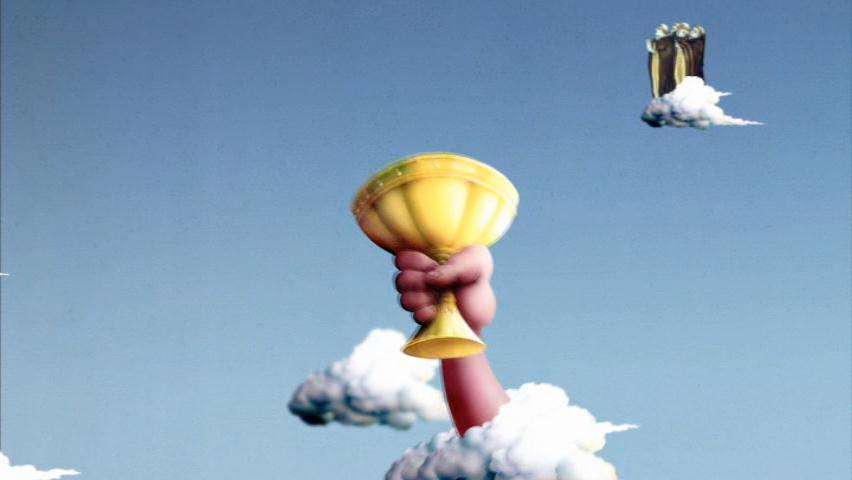
\includegraphics[width=0.8\textwidth]{grail.jpg}
%   \caption[Voorbeeld figuur.]{\label{fig:grail}Voorbeeld van invoegen van een figuur. Zorg altijd voor een uitgebreid bijschrift dat de figuur volledig beschrijft zonder in de tekst te moeten gaan zoeken. Vergeet ook je bronvermelding niet!}
% \end{figure}
% 
% \begin{listing}
%   \begin{minted}{python}
%     import pandas as pd
%     import seaborn as sns
% 
%     penguins = sns.load_dataset('penguins')
%     sns.relplot(data=penguins, x="flipper_length_mm", y="bill_length_mm", hue="species")
%   \end{minted}
%   \caption[Voorbeeld codefragment]{Voorbeeld van het invoegen van een codefragment.}
% \end{listing}
% 
% \lipsum[7-20]
% 
% \begin{table}
%   \centering
%   \begin{tabular}{lcr}
%     \toprule
%     \textbf{Kolom 1} & \textbf{Kolom 2} & \textbf{Kolom 3} \\
%     $\alpha$         & $\beta$          & $\gamma$         \\
%     \midrule
%     A                & 10.230           & a                \\
%     B                & 45.678           & b                \\
%     C                & 99.987           & c                \\
%     \bottomrule
%   \end{tabular}
%   \caption[Voorbeeld tabel]{\label{tab:example}Voorbeeld van een tabel.}
% \end{table}


%%=============================================================================
%% Methodologie
%%=============================================================================

\chapter{\IfLanguageName{dutch}{Methodologie}{Methodology}}%
\label{ch:methodologie}

%% TODO: In dit hoofstuk geef je een korte toelichting over hoe je te werk bent
%% gegaan. Verdeel je onderzoek in grote fasen, en licht in elke fase toe wat
%% de doelstelling was, welke deliverables daar uit gekomen zijn, en welke
%% onderzoeksmethoden je daarbij toegepast hebt. Verantwoord waarom je
%% op deze manier te werk gegaan bent.
%% 
%% Voorbeelden van zulke fasen zijn: literatuurstudie, opstellen van een
%% requirements-analyse, opstellen long-list (bij vergelijkende studie),
%% selectie van geschikte tools (bij vergelijkende studie, "short-list"),
%% opzetten testopstelling/PoC, uitvoeren testen en verzamelen
%% van resultaten, analyse van resultaten, ...
%%
%% !!!!! LET OP !!!!!
%%
%% Het is uitdrukkelijk NIET de bedoeling dat je het grootste deel van de corpus
%% van je bachelorproef in dit hoofstuk verwerkt! Dit hoofdstuk is eerder een
%% kort overzicht van je plan van aanpak.
%%
%% Maak voor elke fase (behalve het literatuuronderzoek) een NIEUW HOOFDSTUK aan
%% en geef het een gepaste titel.

\lipsum[21-25]



% Voeg hier je eigen hoofdstukken toe die de ``corpus'' van je bachelorproef
% vormen. De structuur en titels hangen af van je eigen onderzoek. Je kan bv.
% elke fase in je onderzoek in een apart hoofdstuk bespreken.

%\input{...}
%\input{...}
%...

%%=============================================================================
%% Conclusie
%%=============================================================================

\chapter{Conclusie}%
\label{ch:conclusie}

% TODO: Trek een duidelijke conclusie, in de vorm van een antwoord op de
% onderzoeksvra(a)g(en). Wat was jouw bijdrage aan het onderzoeksdomein en
% hoe biedt dit meerwaarde aan het vakgebied/doelgroep? 
% Reflecteer kritisch over het resultaat. In Engelse teksten wordt deze sectie
% ``Discussion'' genoemd. Had je deze uitkomst verwacht? Zijn er zaken die nog
% niet duidelijk zijn?
% Heeft het onderzoek geleid tot nieuwe vragen die uitnodigen tot verder 
%onderzoek?

\lipsum[76-80]



%---------- Bijlagen -----------------------------------------------------------

\appendix

\chapter{Onderzoeksvoorstel}

Het onderwerp van deze bachelorproef is gebaseerd op een onderzoeksvoorstel dat vooraf werd beoordeeld door de promotor. Dat voorstel is opgenomen in deze bijlage.

%% TODO: 
%\section*{Samenvatting}

% Kopieer en plak hier de samenvatting (abstract) van je onderzoeksvoorstel.

% Verwijzing naar het bestand met de inhoud van het onderzoeksvoorstel

\section{Inleiding}
\label{sec:inleiding}

% Voor wie doen we dit? Wat doet Stater?
Het bedrijf Stater is een end-to-end dienstverlener voor zowel hypothecaire en consumentenkredieten, ze ondersteunen de kredietverstrekker voor de dienstverlening aan consumenten.
% Welke relevante technologie gebruiken ze?
Binnen het bedrijf zijn er verschillende applicatie dat gebruik maken van het Angular framework.
% Wat is Angular?
Angular is een open-source front-end framework, gebaseerd op de TypeScript programmeertaal, dat gebruikt wordt voor de ontwikkeling van dynamische web applicaties \autocite{Cincovic2019}.
% Wat moet er gebeuren? 
Momenteel is Angular versie 20 (v.20) de meest recente stabiele versie.
Binnen Stater maken de applicaties gebruikt van Angular versie 16 (v.16), maar het bedrijf is van plan de applicaties te updaten naar de recentste versie, Angular v.20.

% Waarom moeten de applicaties geupdate worden?
\textcite{Vaniea2016} omschrijven software updates als het introduceren van nieuwe functionaliteiten, de performantie van de applicatie verbeteren en verzekeren dat de software compatibel blijft met nieuwe software en hardware.
Verder omschrijft deze brond dat het up-to-date houden van software cruciaal voor de cyberveiligheid te garanderen.

% Waarom is dit een probleem?
Vanwege het grote verschil in versies zal het updaten van alle applicaties veel tijd in beslag nemen.
% Waarom automatiseren?
Volgends \textcite{Kaur2015} neemt het onderhoudt van een softwareproject gemiddeld 60\% van de kostprijs in beslag.
Een manier om de tijd voor software-onderhoud in te korten is daarom best interesant.
% Wat is de onderzoeksvraag?
Hieruit komt de vraag: In welke mate is het mogelijk om een applicatie in Angular v.16 automatisch te updaten naar Angular v.20?
% In welke deelvragen wordt de onderzoeksvraag opgesplitst?
Voor deze vraag te beantwoorden worden volgende deelvragen geformuleerd:
\begin{itemize}
  \item Wat zijn de veranderingen tussen Angular v.16 en Angular v.20?
  \item Welke van deze veranderingen kunnen automatisch uitgevoerd worden zonder de functionele en niet-functionele vereisten van de applicatie in drang te brengen?
  \item Wat zijn de manieren om code automatisch aan te passen?
  \item Welke manier(en) is meest geschikt voor toe te passen in deze context?
\end{itemize}

% Wat zal gebeuren om de onderzoeksvraag op te lossen?
Gedurende dit onderzoek zal een applicatie ontwikkeld worden dat een software project in Angular v.16 automatisch update naar Angular v.20.
In de rest van dit document wordt naar deze applicatie verwezen als de ``updater''.
% Wat zal de updater doen?
De updater doorloopt de broncode van een applicatie en maakt een oplijsting van alle nodige aanpassingen en tracht de aanpassing zelf uit te voeren indien mogelijk.
% Hoe wordt de updater geëvalueerd?
Voor de effectiviteit van de updater te meten, worden de uit te voeren updates opgedeeld in verschillende categorieën en wordt gemeten hoeveel van de nodige updates automatisch uitgevoerd kunnen worden.

% Wat zal er in de volgende hoofstukken van dit document besproken worden?
In de volgende sectie wordt een kort overzicht gegeven van de huidige stand van zaken binnen het probleem en oplossingsdomein.
Hierna volgt een beschrijving van de methodologie waar de werking en evaluatie van de updater in meer detail beschreven worden.
En tenslotte worden de verwachte resultaten besproken, waarin een inschatting wordt gegeven naar de bevindingen van het onderzoek.

\section{Literatuurstudie}
\label{sec:literatuurstudie}

\subsection{Veranderingen in Angular}

% Wat zijn de aanpassingen die uitgevoert moeten worden?
De \textcite{AngularUpdateGuide2025} geeft ons een uitgebreid overzicht van alle aanpassingen die nodig zijn voor een Angular applicatie van v.16 naar v.20 te updaten. 
Uit deze bron blijkt dat in totaal er 79 verschillende stappen uitgevoerd worden.

De studie door \textcite{Bavota2012} onderzoek welke veranderingen aan code het meeste kans hebben om nieuwe bugs te introduceren.
In deze studie zijn deze verandering onderverdeeld in 4 categorieën: schadelijk, potentieel schadelijk, niet schadelijk en niet geclassificeerd.
Deze studie maakt het mogelijk om een geïnformeerde inschatting te maken naar welke aanpassingen geautomatiseerd kunnen worden zonder onderwachte bijwerkingen te introduceren.

\subsection{Automatisatie process}

% Wat is de meest voor de hand liggende oplossing?
Eén van de meest bekende manieren om code in bulk aan te passen is het gebruik maken van zoek en vervang functies gebaseerd op reguliere expressies (Regex).
Een reguliere expressie is een sequentie van karakters dat een patroon in een tekst omschrijven.
% Wat zijn de problemen bij deze oplossing?
Aangezien dat Regex text gebaseerd is, kan het geen rekening houden met de semantiek van de programmeertaal.
Uit de studie van \textcite{Michael2019} blijken nog enkele problemen bij de implementatie van Regex, namelijk dat het moeilijk leesbaar, vindbaar, valideerbaar en documenteerbaar is.

% Wat is een alternatief?
Om met de semantiek van de programmeertaal rekening te houden kan gebruik gemaakt worden van een abstract syntax tree.
Zoals omschreven door \textcite{Sun2023}, een abstract syntax tree is een data structuur dat de broncode van een applicatie illustreert en rekening houdt met de syntax en semantiek van de programmeertaal.
Dit laat ons toe om een stuk code aan te passen enkel als het in een bepaalde scope zit.

% Is hier al een tool voor?
Herinner dat Angular gebaseerd is op de TypeScript programmeertaal.
Een bestaande tool voor TypeScript dat gebruik maakt van een abstract syntax tree is de TypeScript Compiler API.
De studie door \textcite{Reid2023} onderzoekt hoe de TypeScript compiler gebruikt kan worden voor het corrigeren van foutieve code fragmenten. 
Deze studie raad aan om de TypeScript compiler te gebruiken voor statische code analyse vanwege de effectiviteit, accuraatheid en mogelijkheid om foutieve code te detecteren.

% Wat is een alternatief?
Een alternatief op de TypeScript compiler dat ook gebruikt maakt van een abstract systax tree is het TypeScript Language Server Protocol (LSP).
Het LSP, als omschreven door \textcite{Bork2023}, is een open protocol voor gebruik in verschillende code editors of integrated development environments (IDEs) dat programmeertaal specifieke functies voorziet zoals: automatische code aanvullen en code diagnostiek. 
Dezelfde bron omschrijft LSPs als het de facto standaard protocol voor de implementatie van deze functies in IDEs.

% Wat is een alternatief?
Tenslotte is het mogelijk om AI-tools in te zetten voor deze aanpassingen te maken.
Met de recente opkomst van AI-tools dat specifiek gemaakt zijn voor programmeren is het mogelijk om deze taak uit te besteden aan AI.
Uit de studie door \textcite{Hodovychenko2025} blijkt dat AI gedreven tools een gebrek hebben aan transparantie en risico lopen voor de semantiek van de programmeertaal over tijd fout te interpreteren.

\section{Methodologie}
\label{sec:methodologie}

\subsection{Literatuurstudie}
\label{sec:methodologie:literatuurstudie}

% Wat moet eerst onderzocht worden?
Dit onderzoek start met een uitgebreide literatuurstudie naar de verschillen tussen Angular v.16 en Angular v.20.
% Wat krijgen we uit dit onderzoek?
De nodige verandering worden opgelijst en onderverdeeld in verschillende categorieën.
% Waarom hebben we dit nodig?
Deze lijst zal gebruikt worden voor de capaciteiten van de updater te bepalen.

% Wat moet nog onderzocht worden?
Verder wordt onderzocht wat de verschillende manieren zijn om automatisch code te updaten.
% Wat krijgen we uit dit onderzoek?
Eén of meerdere manieren worden verkozen om te implementeren op basis van volgende parameters:
\begin{itemize}
  \item De complexiteit van de implementatie. Een voorkeur wordt gegeven aan het gebruik maken van bestaande tools over het ontwikkelen van nieuwe algoritme.
  \item De betrouwbaarheid van de output. Is het mogelijk om een correct configuratie een incorrecte output te krijgen?
\end{itemize}

% Hoe lang duurt dit?
Deze literatuurstudie neemt één tot twee weken in beslag en het resultaat dient als basis voor de volgende fase van het onderzoek.

\subsection{Ontwikkeling}

% Wat wordt ontwikkeld?
In deze fase van het onderzoek zal de updater ontwikkeld worden op basis van de voorafgaande literatuurstudie.

% Wat doet de updater?
De updater heeft drie functies: het detecteren van aanpassingen in de broncode, het evalueren of deze aanpassingen automatisch kunnen uitgevoerd worden, en de aanpassingen uitvoeren indien mogelijk.
Elke gedetecteerde aanpassing wordt geregistreerd, waaronder de locatie in de broncode, de aard van de wijziging, de categorie, en of de updater in staat is om de wijziging automatisch uit te voeren.

% Hoe wordt het getest?
De updater wordt in een gecontroleerde omgeving getest om de stabiliteit te verzekeren.
% Hoelang duurt dit?
Voor het ontwikkelen van de applicatie wordt vier tot vijf weken voorzien.

\subsection{Evaluatie}

% Hoe krijgen we resultaten?
De updater wordt uitgevoerd op één van de applicatie binnen Stater.
% Wat doen we met deze resultaten?
Vervolgens wordt het resultaat van de updater geëvalueerd aan de hand van het aantal uitgevoerde aanpassingen ten opzichte van het totaal aantal gedetecteerde aanpassingen.

\section{Verwacht resultaat, conclusie}
\label{sec:verwachte_resultaten}

% Wat zijn de verwachtingen?
Op basis van de literatuurstudie en de gehanteerde methodologie verwacht dit onderzoek dat minstens 75\% van alle nodige aanpassingen automatisch uitgevoerd kunnen worden.
% Wat hebben we hieraan?
Het automatisatie proces zal naar verwachting de nodige tijd voor de applicaties te updaten verminderen.
De hoeveelheid tijd dat in totaal bespaard zal worden zal afhangen van het aantal applicatie en de grootte van de broncode dat geüpdatet moet worden.
Het ontwikkelen van de updater heeft uiteraard ook tijd in beslag genomen.
Deze oplossing zal wellicht meer tijd in beslag nemen als enkel één kleine applicatie geüpdatet moet worden.

% Wat kan nog onderzocht worden?
Of dit de meest effectieve manier is voor deze casus op te lossen is open voor debat.
Verder onderzoek zal uitgevoerd worden naar de performantie, accuraatheid en complexiteit van de verschillende implementaties besproken in de literatuurstudie.



%%---------- Andere bijlagen --------------------------------------------------
% TODO: Voeg hier eventuele andere bijlagen toe. Bv. als je deze BP voor de
% tweede keer indient, een overzicht van de verbeteringen t.o.v. het origineel.
%\input{...}

%%---------- Backmatter, referentielijst ---------------------------------------

\backmatter{}

\setlength\bibitemsep{2pt} %% Add Some space between the bibliograpy entries
\printbibliography[heading=bibintoc]

\end{document}
